\section{Introduction}
With enterprises increasingly adopting Knowledge Graphs (KGs) as the foundation for managing data and building intelligent agents for search, recommendation, and conversation, among others, graph-centered data science is practiced more and more within organizational workflows~\cite{gutierrez2021knowledge}.
These workflows involve iterative and human-centered tasks such as new knowledge acquisition and recommendation, knowledge integration, and curation of the modeled information~\cite{ilyas2022saga, bharadwaj2017creation, knowledgevault, haase2019metaphactory}. 
Therefore, supporting these workflows require experts such as data scientists to blend programming with interactive exploration.
While computational notebooks are suitable for supporting such workflows, the implications of instrumenting programmable and interactive interfaces 
for workflows involving knowledge graphs is underexplored.
% To this end, research on human-centered data science has been exploring various objectives: studying user experiences surrounding data science tools~\cite{chattopadhyay2020s,rahman2020leam,wongsuphasawat2019goals,rahman2021noah}; providing guidelines for workflow authoring paradigms that balance expressivity and ease-of-use~\cite{futzing2019moseying, wu2020b2, bauerle2022symphony, kery2020mage}; reasoning about human agency vs. automation~\cite{zhang2020data, rahman2022ie, heer2019agency}; investigating aspects such as collaboration and reproducibility~\cite{batch2017interactive, zhang2020data, rahman2022ie, Kery2018InteractionsFU, kery2019towards36}; and outlining solutions to address the observed challenges and instrument the recommended guidelines within practical systems~\cite{wu2020b2, bauerle2022symphony, kery2020mage,rahman2020leam}. 
% However, how these observations, guidelines, and solutions apply to data science workflows involving graph exploration and analysis warrants further investigation.

% \begin{figure}[] 
%   \centering
%   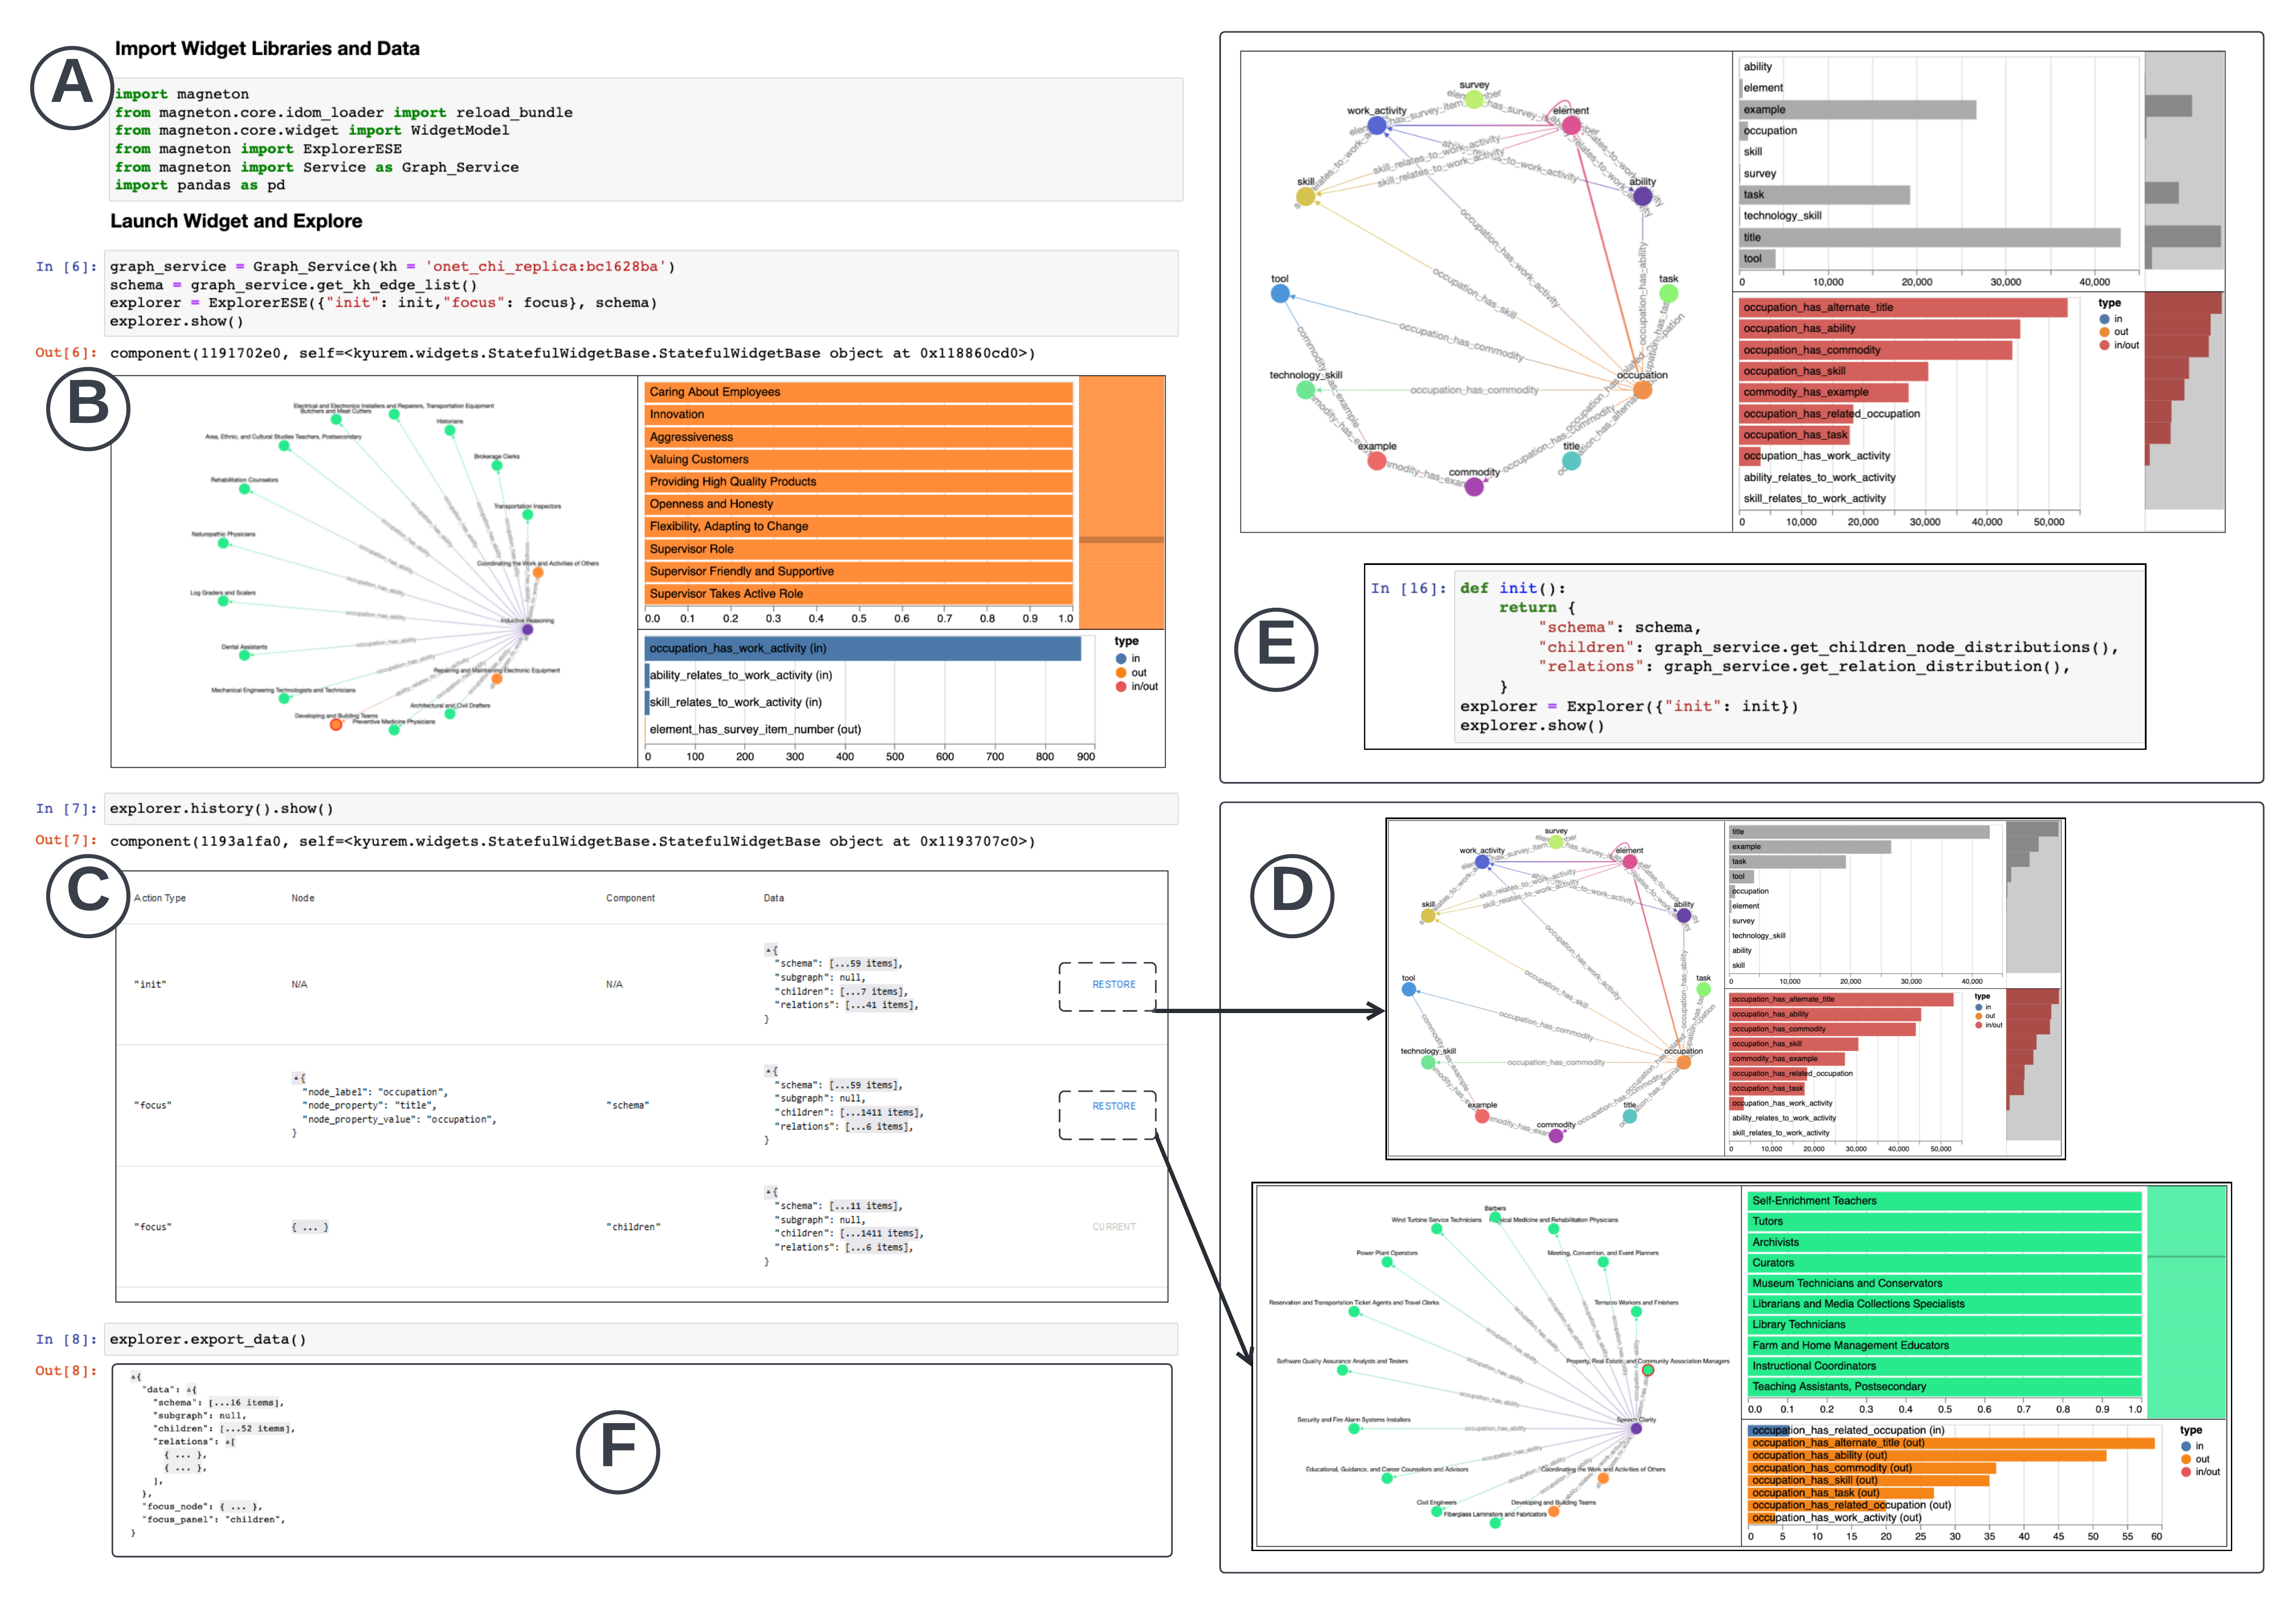
\includegraphics[width=\linewidth]{figures/teasersecond.png}
%   \caption{Overview of \system features. (A) An example data science notebook involving knowledge graph exploration using \system. User first imports the \system library and data. (B) User then launches an exploration widget to explore the graph within a multiple-coordinated view component using various interactions such as semantic zooming and selection. User obtains additional details about the graph entity type such as other similar entities in the graph and the degree (both in and out) distribution of relations corresponding to an entity. (C) User chooses to view their exploration history using the provenance viewer of the exploration widget. (D) By clicking the \emph{Restore} button, they explore the data states corresponding to various actions. (E) User defines a custom intialization function in the notebook to sort the top right distriubtion in alphabetic order, (F) User selects one of the states containing relevant information to share with the other team members. To do so, the user exports the corresponding data which can
%   be further viewed and explored within a hierarchical data viewer component. We included a video demo of \system in supplementary material.}
%   \label{fig:teaser} 
% \end{figure}

% \begin{figure}[!htb] 
%   \centering
%   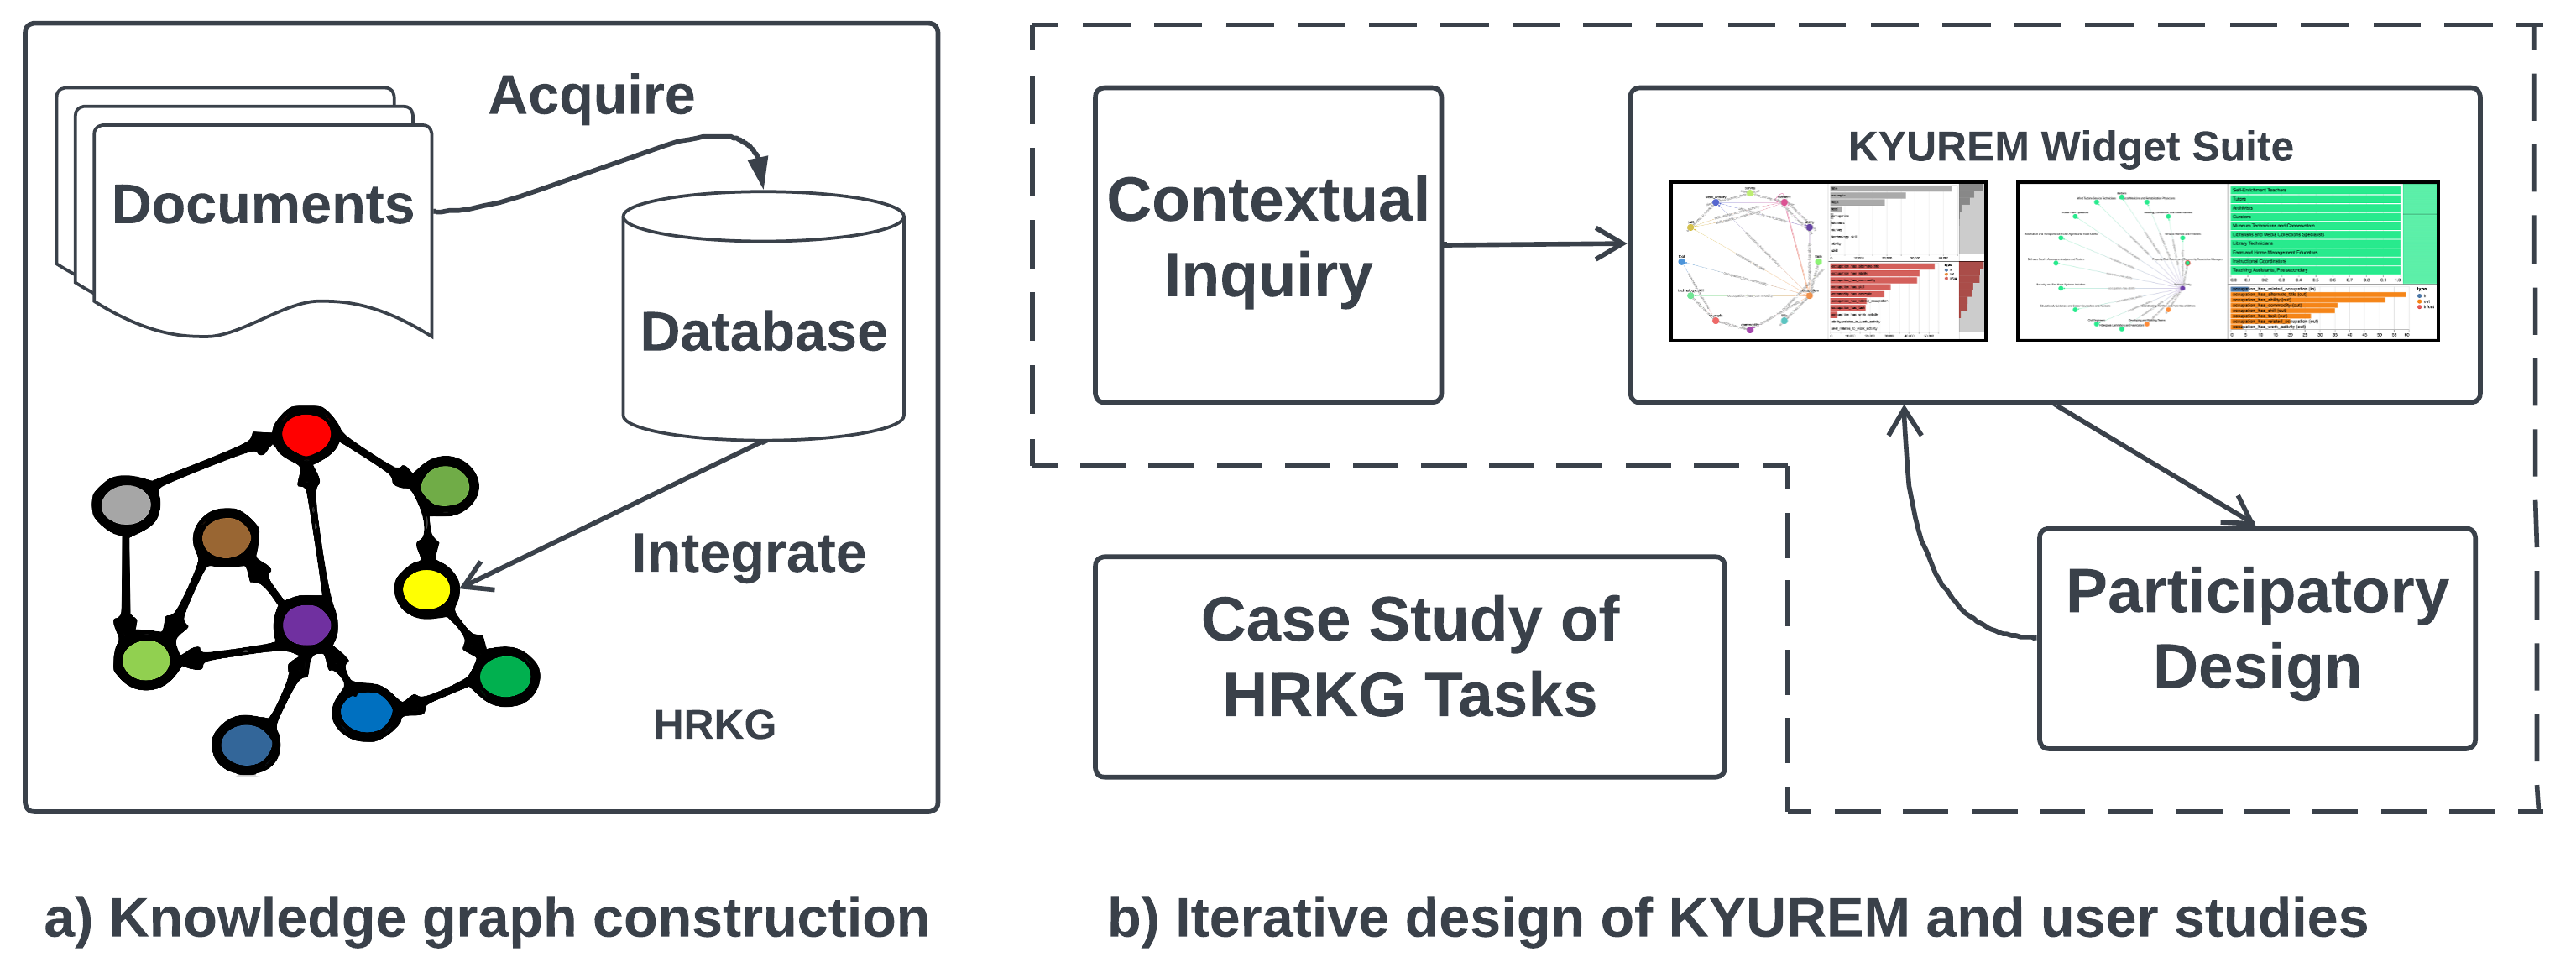
\includegraphics[width=0.5\linewidth]{figures/workflow.png}
%   \vspace{-10pt}
%   \caption{An overview of the \company HRKG tasks, the corresponding user study design, and eventual \system library.}
%   \vspace{-10pt}
%   \label{fig:workflow} 
% \end{figure}

\begin{figure*} 
\vspace{-10pt}
    \centering
  \subfloat[\label{fig:overview}]{%
       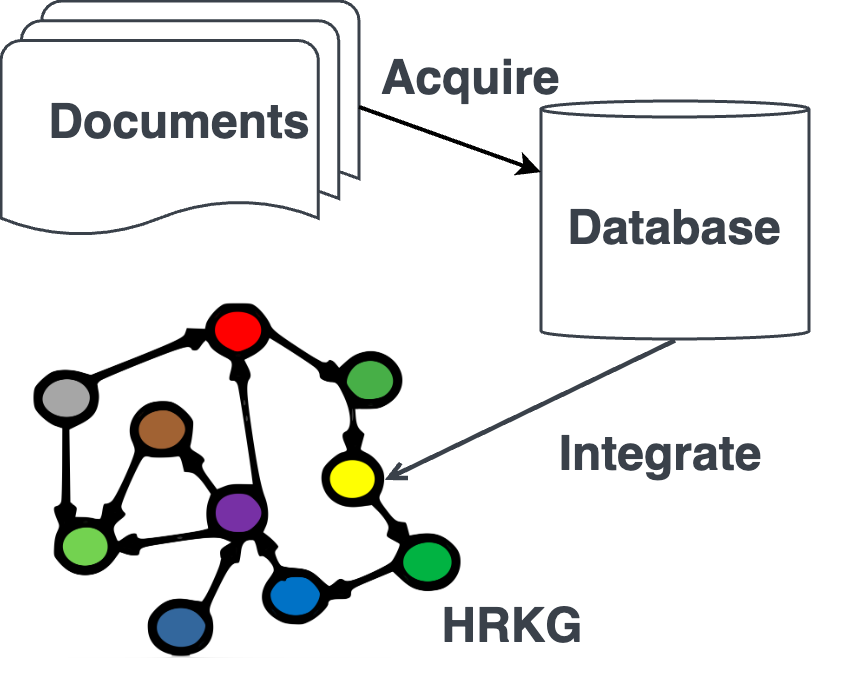
\includegraphics[width=0.18\linewidth]{figures/hrkg.drawio.png}}
    \hfill
  \subfloat[\label{fig:study_flow}]{%
        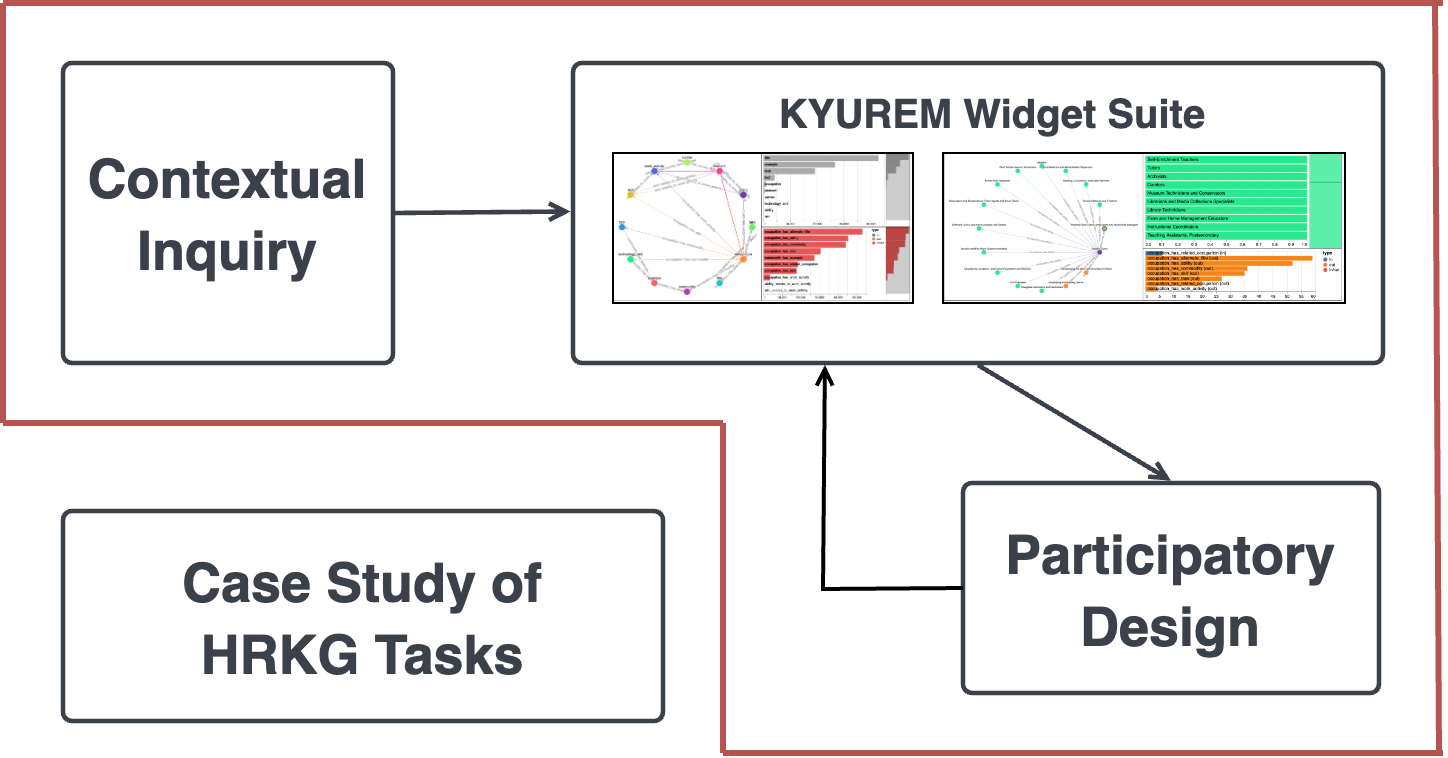
\includegraphics[width=0.28\linewidth]{figures/study-flow.drawio.png}}
    \hfill
  \subfloat[\label{fig:archi}]{%
        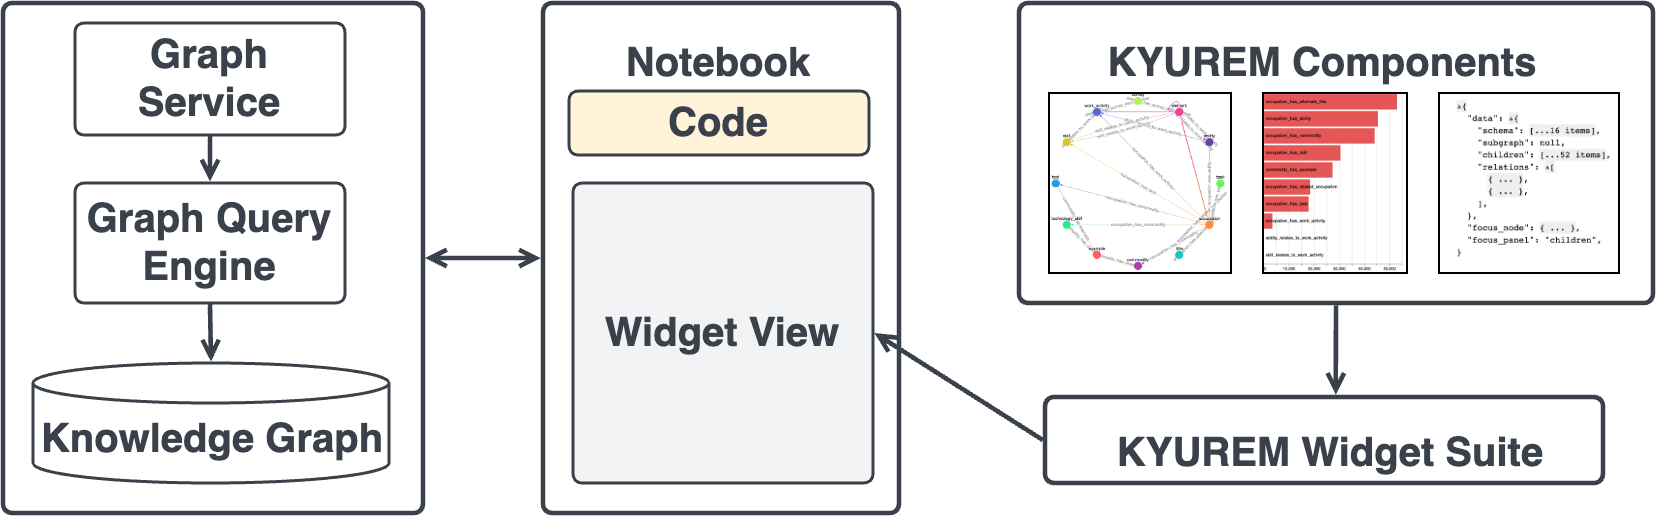
\includegraphics[width=0.48\linewidth]{figures/kyurem-archi.drawio.png}}
  \caption{(a) An overview of the \company HRKG tasks, (b) the study design, and (c) the \system system architecture.}
  \label{fig:overview} 
\vspace{-10pt}
\end{figure*}

In this work, we focus on two specific tasks within the human resources knowledge graph (HRKG hereafter) construction and serving platform at \company --- knowledge acquisition and knowledge integration, an industrial lab focusing on natural language processing, data management, and human-centered AI research. 
\company is a subsidiary of a large holding and conducts research and development for the other subsidiaries with worldwide businesses in staffing, human resources, travel, marketing, and other online consumer services.
Knowledge graph (KG) construction and serving plays a central role at \company. 
Deploying and maintaining a KG that can be shared across 
applications has obvious benefits, as applications such as QA systems, search engines, 
conversational agents~\cite{quamar2020ontology}, and training large language models~\cite{zhao2021knowledge}
require accurate and up-to-date facts about entities and relations. 
% For instance, open-domain knowledge powers the question-answering 
% capabilities of search engines and conversational AI~\cite{quamar2020ontology}. 
% Moreover, KGs are reliable sources of training datasets
% for machine learning and 
% natural language processing workflows~\cite{ji2021survey}.
% The structured information encoded in graphs
% has been shown to complement large language models in
% various applications~\cite{zhao2021knowledge}. 
Therefore, facilitating a broad range of knowledge that is accurate
and updated continuously is of utmost importance. The HRKG platform
at \company is similar to other such platforms
in industry~\cite{ilyas2022saga, bharadwaj2017creation, knowledgevault, haase2019metaphactory},
where, information about entities is obtained by integrating data from multiple 
structured (\eg relational databases, taxonomies, other KGs) and unstructured sources (\eg documents, web text)~\cite{chen2020kgpt}.


As shown in Figure~\ref{fig:overview}, the KG construction and maintenance involves various tasks from knowledge acquisition to
knowledge integration and canonicalization.
All of these steps involve multiple stakeholders (\eg engineers, researchers, taxonomy architects)
and require significant human intervention. 
Within the KG construction and serving workflow, data practitioners face many challenges. To better understand the challenges and to provide meaningful solutions we conducted several studies within \company (see Figure~\ref{fig:study_flow}.)
We conducted a contextual inquiry-style study~\cite{holtzblatt1997contextual}, where we observed the work practices of three data practitioners working on projects related to knowledge acquisition and integration within the HRKG platform. The study helped understand the pain points of the practitioners and informed design guidelines to assist the experts in performing knowledge acquisition and integration within the HRKG. One such example is the negative user experience with existing tools stemming from frequent context switching to accommodate multiple objectives, \eg programming, and visualization. Using programmable and interactive interfaces integrated with Computational notebooks (\eg Jupyter~\cite{kluyver2016jupyter} and Observable~\cite{observable}) may minimize such context switching.

% We noticed similarities between our observed challenges and the reported challenges in human-centered data science research mentioned earlier. One such example is the negative user experience with existing tools stemming from frequent context switching to accommodate multiple objectives, \eg programming, and visualization. Using programmable and interactive interfaces integrated with Computational notebooks (\eg Jupyter~\cite{kluyver2016jupyter} and Observable~\cite{observable}) may minimize such context switching.  Data practitioners
% employ these interfaces for auditing, reproducing, or sharing data insights~\cite{wu2020b2,bauerle2022symphony,kery2020mage, rahman2020leam}. 

%However, gaps remain with respect to reproducibility, reusability, and customizability of user actions as users accomplish graph exploration and analysis using these interfaces. These gaps stem from the design of programmable and interactive interfaces and are further exacerbated when observed within an organizational workflow. 



% In particular, current programmable and interactive interfaces are essentially lightweight visualization tools where a user action on the interface triggers data operations that update the interface's state and initiate a re-render of the interface. 
% However, existing solutions do not instrument principled provenance management to track fine-grained user actions and their corresponding states as popular data exploration tools like Tableau~\cite{tableau} and  PowerBI~\cite{powerbi}. Moreover, the lack of a tight coupling between the interfaces and the underlying state management mechanisms makes it difficult to access and reuse arbitrary states from users' interaction history. Furthermore, these interfaces lack the affordances for customizing built-in data operations that update interface states when triggered by user actions. For example, a search operation over a dataframe column containing textual data --- triggered via interaction on the corresponding visualization --- is pre-defined and cannot be modified by a user to accommodate other objectives such as semantic search by synonyms or POS tags~\cite{rahman2022ie}. Finally, these interfaces currently lack support for authoring interactive workflows involving knowledge graph exploration and analysis as they prioritize other data domains such as tables, text, and images. 

% \danc{is \system restricted to KG exploration?}

% \sajc{yes. for now. In Section~\ref{sec:discuss} we will discuss generalizabiliy.}

% \hkc{why are these existing gaps important in KG exploration? e.g., capturing provenance is essential in KG workflow; KG analysis requires various kinds of zooming-in (by node, by relation, etc?) thus the need for customization}
% \sajc{made updates. please review}



% \footnote{Similar to Magneton, a robot-like Pok\'emon, our proposed framework stitches together three objectives (Magnemite): provenance, reusability, and customization, to enable robust \emph{programmable and interactive} interfaces in computational notebooks.}, a framework for creating and composing programmable and interactive interfaces 
% equipped with built-in provenance and on-demand customization capabilities. \dan{}{These interfaces are developed by extending widgets in computational notebooks such as  \emph{ipywidgets}~\cite{IPyWidgets}.
% The interface consists of a built-in interaction-aware state manager and a persistent provenance manager to ensure reusability and reproducibility of actions.} Moreover, an augmented communication manager enables sharing of user-defined functions between notebooks and widgets to facilitate customization of data operation. 

To address these gaps, we implement \system widget suite --- a library of interactive widgets built using the \basesystem framework~\cite{choi2023towards} --- to specifically support expert-in-the-loop knowledge acquistion and integration tasks. The in-notebook widgets display task-specific visualizations and support user interactions on the interface. The task-specific visualizations and their corresponding interactions are implemented based on design guidelines identified from existing work on graph visualization and exploration~\cite{liu2018graph, 2019_eurovis_mvnv, pienta2015scalable, pretorius2014tasks, kerracher2015task, ahn2013task, lee2006task}. To enable graph-centric data science, we build a python library that translates user interactions on the widgets to graph queries. 
% As shown in Figure~\ref{fig:teaser}, users author their workflows in the Jupyter notebook by loading data and instantiating task-specific widgets. Each widget has a built-in provenance viewer, enabling users to explore their interaction history with additional contextual information. Users can customize an interaction's underlying data operation by writing custom code in the notebook and passing those as callback functions during widget instantiation. Finally, users can export any widget state using the provenance view to interactively revisit previous actions and then leverage data accessors to export the desired information. The exported data can then be reused in subsequent steps, other projects, or loaded into another widget for follow-up analysis. 
We worked with $12$ data practitioners (\eg researchers, engineers, and data scientists) at \company in weekly participatory design sessions over six weeks to further understand their requirements. Informed by these sessions, we implemented additional \system widgets and components
supporting tasks such as new knowledge acquisition and acquired knowledge integration. Finally, we conducted two case studies to understand the implications of instrumenting \system within the in-house HRKG platform. The experience of the experts-in-the-loop were positively impacted by the introduction of \system. Participants also found new insights that were previously not apparent to them due to the absence of interactive interfaces, such as data quality issues with the knowledge acquisition tasks.

% The key contributions of this work are as follows: 
% \begin{itemize}
%     \item We developed \system, a framework for composing interactive interfaces within computational notebooks that enable reproducible, reusable, and customizable workflows involving graphs.
%     \item We launched contextual inquiries to motivate the design goals of \system, organized participatory design sessions for augmenting and focusing the design of \system widgets and conducted case studies on three real-world projects within an industry setting.
%     \item The analysis of the study results highlighted the benefits of \system and reported discussion on possible extensions to other tasks and workflows. The follow-up discussion highlighted potential future research opportunities spanning several disciplines within computer science.
%      \estevam{\item filled the gap present in current graph exploration tools, which do not support blending codes with visualizations
%       \item supporting the highly iterative workflows while capturing the state of exploration, the provenance of interactions on visualizations, and on-demand customization of interactions}

% \end{itemize}
  
% \system combines the following principles to improve upon programmable and interactive interfaces for data science workflows:
% \begin{itemize}
%     \item \textbf{Robust interaction provenance.} Track the interaction state as well as the visualization state and ensure appropriate mapping among interaction and visualization states and data operations. 
%     \item \textbf{Reusable components.} Persist visualization states and provide mechanisms to access any states within user's current analytics session. 
%     \item \textbf{Customization of interaction outcomes.}
% Enable users to customize the data operation underlying a visual interaction to provide more flexibility in meeting their analytics goal.
% \end{itemize}
% \hkc{current principles are more about general EDA in notebooks. (for better flow)ground principles in KG workflows and mention that these principles are also applicable to any non-KG exploration workflow.}




% \begin{figure}[!htb] 
%   \centering
%   \includegraphics[width=0.8\linewidth]{figures/ds_workflow.png}
%   \caption{An iterative graph analysis workflow consisting of data loading, overviewing, navigation, and decision making.}
%   \label{fig:ds_workflow} 
%   \Description{Place holder figure.}
% \end{figure}



